


\begin{figure*}
  \jsubfig{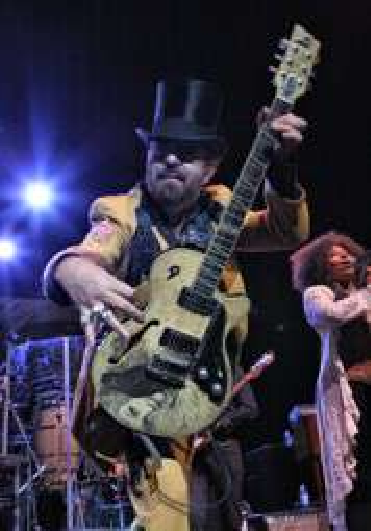
\includegraphics[height=4.3cm]{figures/hhi_example.pdf}}
  {\vspace{-5pt}\begin{center} \small{(a) 
  
  [*] performing with [*]} \end{center}}
  \hfill
  \jsubfig{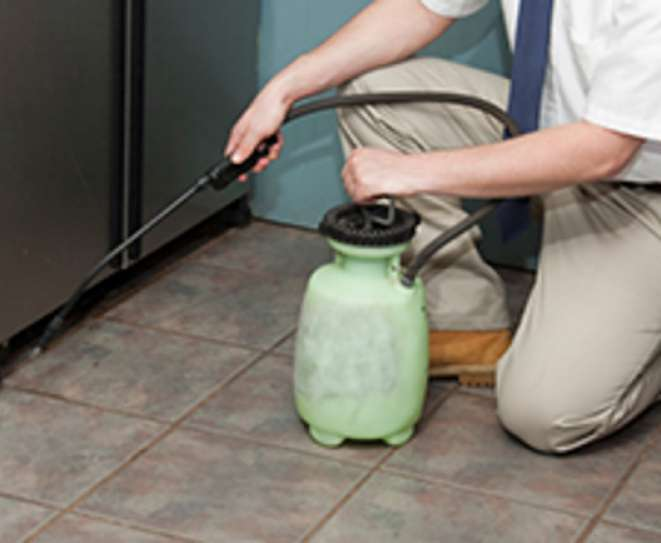
\includegraphics[height=4.3cm]{figures/sir_example.pdf}}
  {\vspace{-5pt}\begin{center} \small{(b)\\ VERB exterminating AGENT man INSTRUMENT nozzle PLACE floor} \end{center}}
  \hfill
  \jsubfig{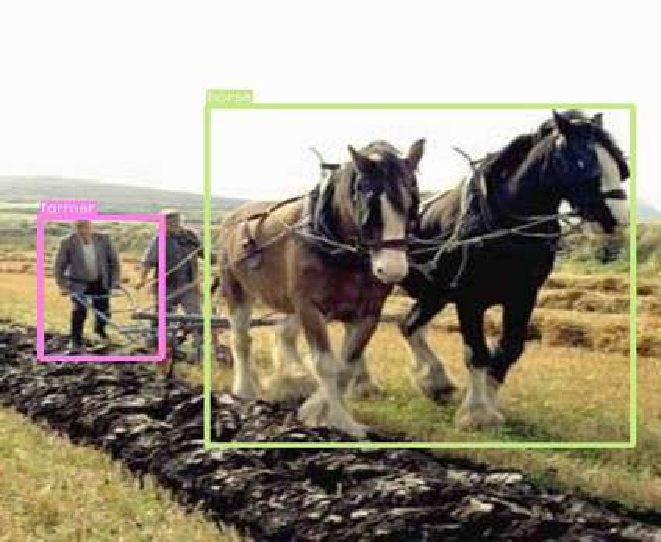
\includegraphics[height=4.3cm]{figures/gsr_example.pdf}}
  {\vspace{-5pt}\begin{center} \small{(c)
\\ VERB plowing AGENT farmer INSTRUMENT horse PLACE field} \end{center}}
  \hfill
  \jsubfig{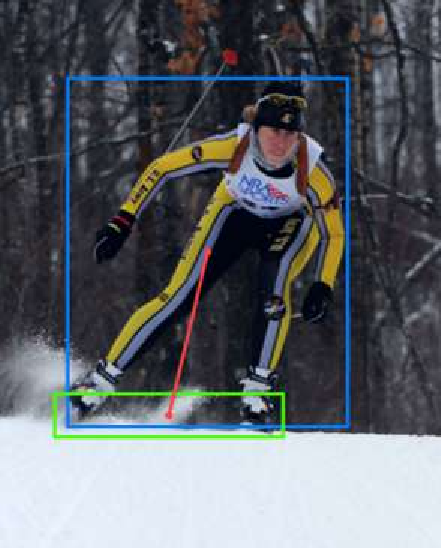
\includegraphics[height=4.3cm]{figures/hoi_example.pdf}}
  {\vspace{-5pt}\begin{center} \small{(d)\\ride; stand on; wear} \end{center}}
  
  \caption{\textbf{Qualitative results.} 
  Results of our framework over several dynamic scene understanding tasks: \textbf{(a)} Human-Human Interaction (HHI), \textbf{(b)} Situation Recognition (SiR), \textbf{(c)} Grounded Situation Recognition (GSR), and \textbf{(d)} Human-Object Interaction Detection (HOI). For further details on these tasks, see Section \ref{sec:tasks}}   %
\label{fig:all_tasks_result}
\end{figure*}
